\chapter{Strategie di ricerca}

Il presente capitolo è dedicato all'implementazione in Prolog di alcune tipiche strategie di ricerca nello spazio degli stati. Il dominio scelto per testare la correttezza e valutare le prestazioni degli algoritmi realizzati è quello del mondo dei blocchi. Segue una descrizione di come è stata affrontata la modellazione del problema, delle scelte implementative e dei test effettuati con i relativi benchmark.

\section{Modellazione ed implementazione}
 
\subsection{Rappresentazione degli stati}
Seguendo la traccia proposta, si è deciso di rappresentare un generico stato per mezzo di un insieme ordinato di predicati che descrivono la situazione corrente. Utilizzare un insieme ordinato permette di confrontare gli stati e stabilirne l'uguaglianza in modo efficiente; l'efficienza rappresenta un fattore importante in quanto il suddetto controllo serve per distinguere gli stati già visitati da quelli nuovi, ed è pertanto molto frequente. 

\subsection{Modelli di transizione}
Sono stati utilizzati due diversi modelli di transizione che si differenziano soprattutto per la presenza o meno di una restrizione riguardante il numero di pile che è consentito costruire.\\

\noindent\textbf{Modello di transizione A}\\
Il primo modello non pone alcun limite al numero di blocchi che possono essere direttamente posizionati sul tavolo: è pertanto possibile formare tante pile quanti sono i blocchi (ogni pila sarà ovviamente composta da un unico blocco).
Le azioni possibili secondo questo primo modello di transizione sono in totale quattro: 
\[ pickup(X), putdown(X),stack(X,Y),unstack(X,Y) \]
I predicati utilizzati per descrivere un generico stato sono invece:
\[ on(X,Y),clear(X),ontable(X),holding(X),handempty \]
dove in entrambi i casi $X$ e $Y$ rappresentano dei blocchi.\\

\noindent\textbf{Modello di transizione B}\\
È facile convincersi che, utilizzando la modellazione precedentemente descritta, è possibile risolvere qualsiasi istanza del problema adottando una strategia comune: infatti, è sempre possibile posizionare tutti i blocchi direttamente sul tavolo per poi costruire la configurazione desiderata. In generale, poter disporre di un numero arbitrario di pile semplifica la ricerca di soluzioni.
Si è pertanto scelto di vincolare maggiormente il problema: il modello di transizione è stato riscritto in modo da considerare solo un numero finito di posizioni sul tavolo (che chiameremo per comodità ``pilastri"), secondo una formulazione che ricorda quella della Torre di Hanoi. Allo stesso tempo, sono state riformulate le azioni possibili, che nel presente modello sono soltanto due:
\[ put\_on\_block(X,Y),put\_on\_pillar(X,P)\]
Inoltre, i predicati utilizzati per descrivere un generico stato diventano:
\[ on(X,Y),clear(X),onpillar(X,P),free(P) \]
dove $X$ e $Y$ indicano dei blocchi e $P$ un generico pilastro.

Di fatto, sono state accorpate le azioni che nel modello precedente venivano compiute in due step. La coppia di azioni $unstack(X,Y)$ seguita da $stack(X,Z)$ diventa così, ad esempio, un'unica azione $put\_on\_block(X,Z)$. La semantica rimane ovviamente immutata: il blocco $X$ passa dall'essere posizionato sopra al blocco $Y$ all'essere impilato su $Z$.
Allo stesso modo, $put\_on\_pillar(X,P)$ sostituisce la coppia $unstack(X,Y)$ e $putdown(X)$, aggiungendo informazione riguardante la posizione occupata sul tavolo.
Lo specifico comportamento di un'azione viene stabilito in base alla posizione del blocco a cui viene applicata; si consideri a titolo di esempio l'implementazione di $put\_on\_pillar$:
\lstset{numbers=left,breaklines=true,language=Prolog,basicstyle=\small\ttfamily}
\begin{lstlisting}[frame=single]
applicable(put_on_pillar(X,P),S):-
	block(X),
	pillar(P),
	ord_memberchk(clear(X),S),
	ord_memberchk(free(P),S).

% if X is above another block
transform(put_on_pillar(X,P),S1,S2):-
	member(on(X,Z),S1),!,
	list_to_ord_set([on(X,Z),free(P)],DLS),
	ord_subtract(S1,DLS,S),
	list_to_ord_set([onpillar(X,P),clear(Z)],ALS),
	ord_union(S,ALS,S2).

% if X is above a pillar
transform(put_on_pillar(X,P),S1,S2):-
	member(onpillar(X,R),S1),
	list_to_ord_set([onpillar(X,R),free(P)],DLS),
	ord_subtract(S1,DLS,S),
	list_to_ord_set([onpillar(X,P),free(R)],ALS),
	ord_union(S,ALS,S2).
\end{lstlisting}

Per quanto riguarda la rappresentazione degli stati, non è più necessario disporre del predicato $handempty$ in quanto le azioni sono atomiche: esse partono da una situazione in cui vale $handempty$ e si concludono in una situazione analoga. Implicitamente, si assume che non vengano mai specificati stati goal in cui un blocco viene tenuto in mano. 

È comunque importante notare che disporre di sole due azioni invece che quattro non comporta un vantaggio in termini computazionali: l'unico vantaggio risiede nella compattezza della soluzione, che risulta più leggibile in quanto composta da meno azioni. Inoltre, risulta libera da inutili ``ridondanze": è infatti scontato che, una volta sollevato un blocco, la mossa successiva consisterà nel posizionamento del suddetto blocco sul tavolo o su una pila già esistente.

\subsection{Euristiche}
Poiché due dei tre algoritmi implementati fanno uso di euristiche, una particolare attenzione è stata dedicata alla scelta e all' implementazione delle suddette. Di seguito vengono descritte e confrontate le due euristiche realizzate.\\

\noindent\textbf{Euristica A}\\
La prima euristica è relativamente semplice: restituisce un valore pari al numero di blocchi che non si trovano in goal position. Un blocco viene detto essere in goal position quando tutti i blocchi ad esso sottostanti (fino al tavolo) sono gli stessi e compaiono nel medesimo ordine sia nello stato corrente che nello stato goal. \\

\noindent\textbf{Euristica B}\\
La seconda euristica non si limita a considerare il numero di blocchi che devono essere certamente mossi in quanto non si trovano nella loro posizione finale, bensì stima il numero di azioni che sarà necessario compiere per alterarne opportunamente la posizione. Nello specifico, si effettua una distinzione fra blocchi che dovranno essere mossi almeno una volta, e blocchi che dovranno essere mossi almeno due volte:
\begin{itemize}
\item Un blocco $X$ deve essere mosso almeno una volta se poggia su un blocco differente da quello sul quale si trova nello stato goal (anche un posizionamento errato sul tavolo rientra in questo caso).
\item Un blocco $X$ deve essere mosso almeno due volte se vale una delle seguenti condizioni:
\begin{itemize}
\item X poggia sullo stesso blocco sul quale si trova nello stato finale, ma quest'ultimo deve essere mosso una volta;
\item al di sotto di $X$ (nella stessa pila) vi è almeno un blocco che deve essere mosso due volte.
\end{itemize}
\end{itemize}
La nuova euristica domina la precedente (rimanendo comunque ammissibile) e in alcuni casi arriva a stimare correttamente il numero di passi effettivamente necessari al raggiungimento dello stato goal, come si evince dal grafico riportato in figura \ref{heuristics}. Questa seconda euristica in sostanza risulta essere notevolmente più informata rispetto alla precedente, e ci si attende pertanto che porti a delle prestazioni migliori.

\begin{figure}[h]
\centering
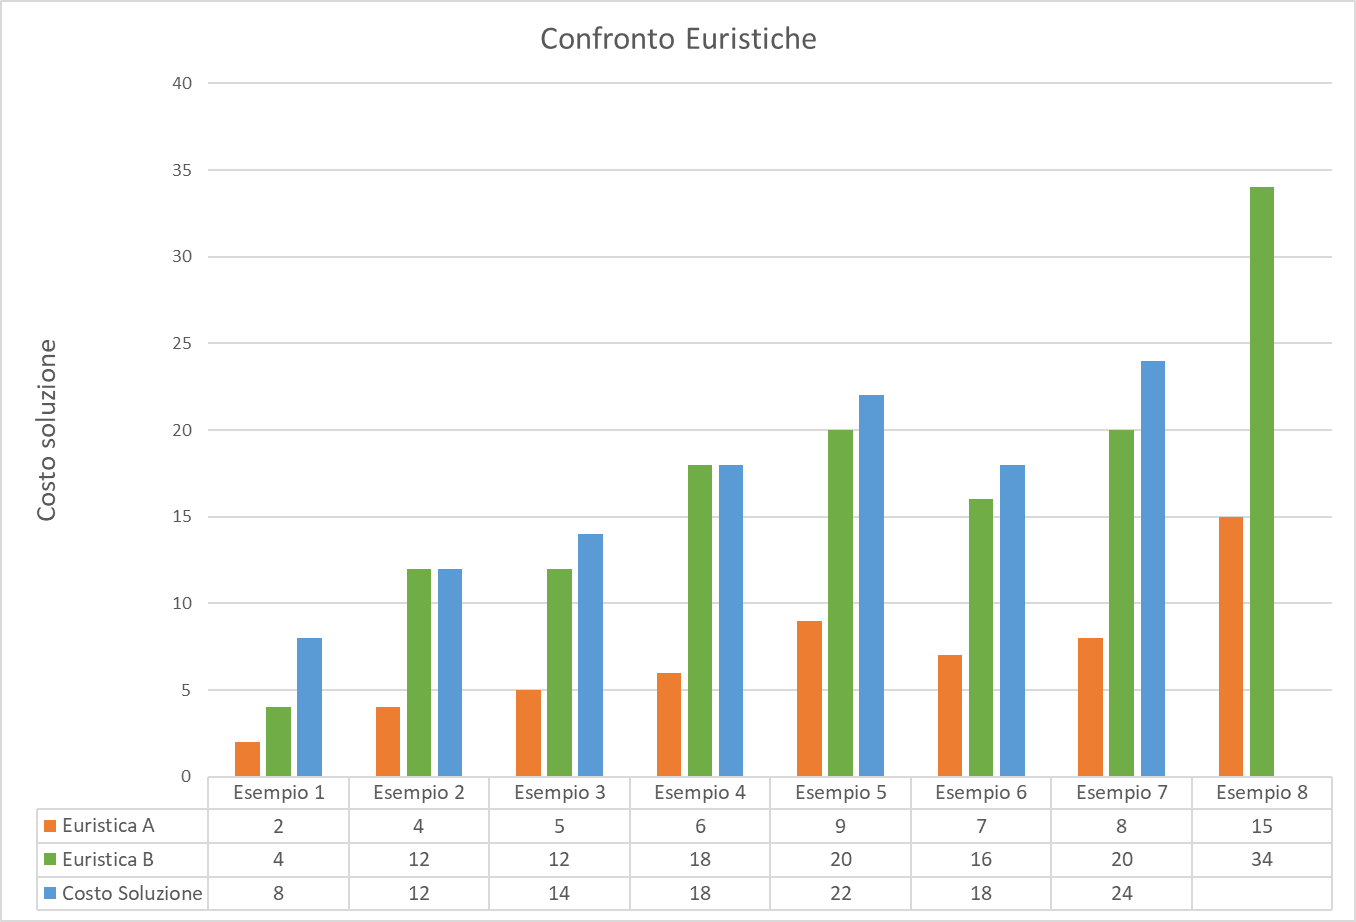
\includegraphics[width=\textwidth]{heuristics}
\caption{Confronto fra euristica A ed euristica B in termini di costi stimati,\\ considerando il modello di transizione A e costi unitari per le tutte le azioni.}
\label{heuristics}
\end{figure}


\subsection{Ulteriori note riguardanti l'implementazione}

\noindent\textbf{Iterative Deepening DFS}\\
In presenza di uno spazio degli stati di cardinalità infinita, e in caso non vi sia soluzione, vengono meno le condizioni di terminazione per qualsiasi algoritmo di ricerca. Per questo motivo, nel caso di Iterative Deepening DFS, viene comunque richiesta all'utente una soglia massima oltre la quale non proseguire ulteriormente la ricerca.\\

\noindent\textbf{\textbf{A\textsuperscript{*}}}\\
L'algoritmo è caratterizzato dalla presenza di una coda di priorità che viene utilizzata per selezionare il nodo avente $f$-$value$ minimo tra quelli marcati come ``Aperti", pertanto la scelta della struttura dati che implementa suddetta coda è un aspetto di cruciale importanza. Attualmente, essa è realizzata mediante una semplice lista ordinata. Questa non è certamente la scelta migliore: sia l'inserimento che l'aggiornamento di un valore risultano infatti avere complessità lineare. Una struttura più adeguata sarebbe uno heap; purtroppo l'implementazione messa a disposizione da $SWI$-$Prolog$ non è abbastanza flessibile per permetterne l'utilizzo in questo contesto. Se infatti l'inserimento risulta certamente più efficiente, lo stesso non si può dire per l'aggiornamento di un valore già presente: sono del tutto assenti procedure che permettano di effettuare operazioni quali ``update\_key" o ``heapify". Il principale miglioramento da apportare in futuro sarebbe quindi la sostituzione della lista ordinata con una struttura dati più efficiente. \\

\noindent\textbf{\textbf{IDA\textsuperscript{*}}}\\
Sono state realizzate due versioni del presente algoritmo. La prima fa uso del predicato \texttt{asserta()} per aggiungere dinamicamente dei fatti a runtime: è così possibile tenere agevolmente traccia del più piccolo $f$-$value$ che ha superato la soglia durante una specifica iterazione. La seconda invece non fa uso del predicato \texttt{asserta()} ed è quindi costretta a ``portarsi dietro", di predicato in predicato, suddetta informazione. Dal punto di vista pratico non sono state registrate differenze di prestazioni significative dovute ai due diversi approcci; la prima versione è quindi da preferire in quanto indubbiamente più leggibile.

\section{Test e confronti}

\subsection{Esempi utilizzati} 
Nella fase di test e di raccolta dei benchmark, ci siamo serviti di vari esempi. Suddetti esempi sono elencati in figura \ref{block_examples}, dove risultano ordinati per complessità e sono associati al relativo numero di passi necessari per essere risolti (nei casi in cui risolvere il problema è stato effettivamente possibile considerando le ovvie limitazioni temporali). 

\begin{figure}[h]
\centering
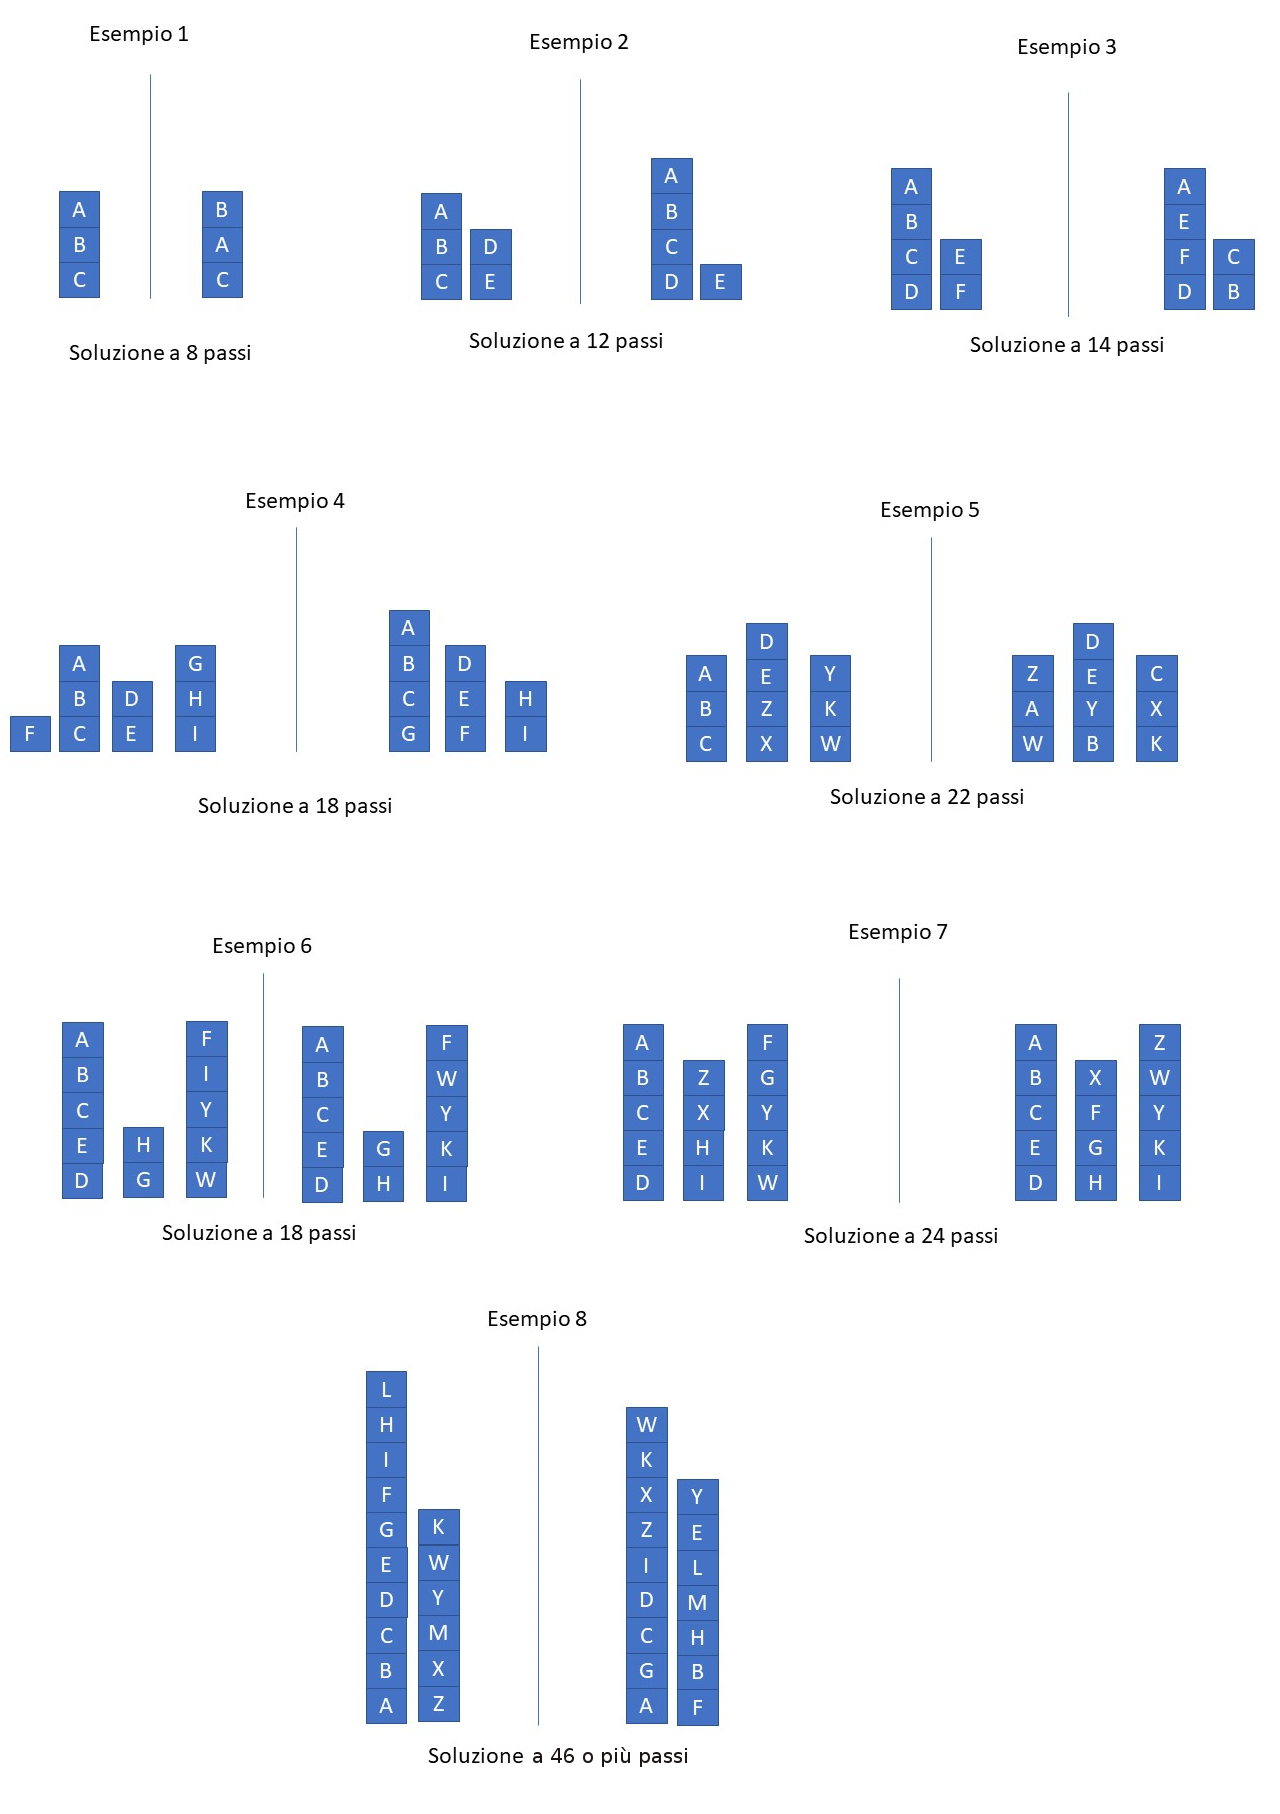
\includegraphics[width=\textwidth]{block_examples}
\caption{Esempi e costo totale delle relative soluzioni (quando note) utilizzando il modello di transizione A.}
\label{block_examples}
\end{figure}

\subsection{Costo non unitario delle azioni}
Uno degli esperimenti condotti è incentrato sul costo delle azioni. La formulazione più comune del dominio considerato prevede un costo unitario uguale per tutte le azioni; tuttavia gli algoritmi sono stati concepiti in modo da garantire all'utente piena libertà nello specificare tali costi. Durante questo test, l'attenzione è stata interamente rivolta verso il modello di transizione A. Infatti, utilizzando il suddetto modello, le soluzioni ottimali prevedono spesso un parziale ``appiattimento" della configurazione, ovvero molti blocchi vengono appoggiati direttamente sul tavolo. Ci si è quindi domandati se aumentare il costo delle azioni \textit{putdown/pickup} potesse limitare significativamente il numero di nuove pile create senza ricorrere a dei vincoli espliciti, come avviene invece nel modello di transizione B. Nello specifico è stato immaginato un contesto in cui $putdown$ ha un costo 4 volte maggiore rispetto alle altre azioni.
I risultati ottenuti hanno confermato quanto ipotizzato: la profondità delle soluzioni ottimali è maggiore (e pertanto è maggiore il tempo di calcolo necessario per trovarle) ma il numero totale di blocchi posizionati direttamente sul tavolo è notevolmente ridotto.
Si riportano le soluzioni ottenute per l'esempio 3 nei due diversi casi:

\begin{itemize}
\item Soluzione considerando azioni di costo unitario: \\
\textit{unstack(e,f), putdown(e), unstack(a,b), putdown(a), unstack(b,c), putdown(b), unstack(c,d), stack(c,b), pickup(f), stack(f,d), pickup(e), stack(e,f), pickup(a), stack(a,e).}
\item Soluzione considerando un costo per $putdown$ 4 volte maggiore: \\
\textit{unstack(a,b), stack(a,e), unstack(b,c), putdown(b), unstack(c,d), stack(c,b), unstack(a,e), stack(a,c), unstack(e,f),
stack(e,a), pickup(f), stack(f,d), unstack(e,a), stack(e,f), unstack(a,c), stack(a,e).}
\end{itemize}

Si noti che nel primo caso lo stato goal viene raggiunto in 14 passi, ma in totale vengono occupate ben 5 posizioni differenti sul tavolo (corrispondenti alle 2 pile iniziali e ai 3 blocchi appoggiati direttamente sul tavolo, ovvero $e,a,$ e $b$) . Nel secondo caso invece la soluzione è a profondità 16, ma solo 3 posizioni sono utilizzate.

\subsection{Confronto delle prestazioni degli algoritmi}
Nelle considerazioni che seguono, si fa riferimento all'immagine \ref{normal_compare} in cui si confrontano il tempo impiegato per trovare una soluzione ed il numero nodi espansi durante la ricerca dai diversi algoritmi. Tutti i risultati sono stati ottenuti facendo uso del modello di transizione A e dell'euristica B.\\

\begin{figure}[h]
\centering
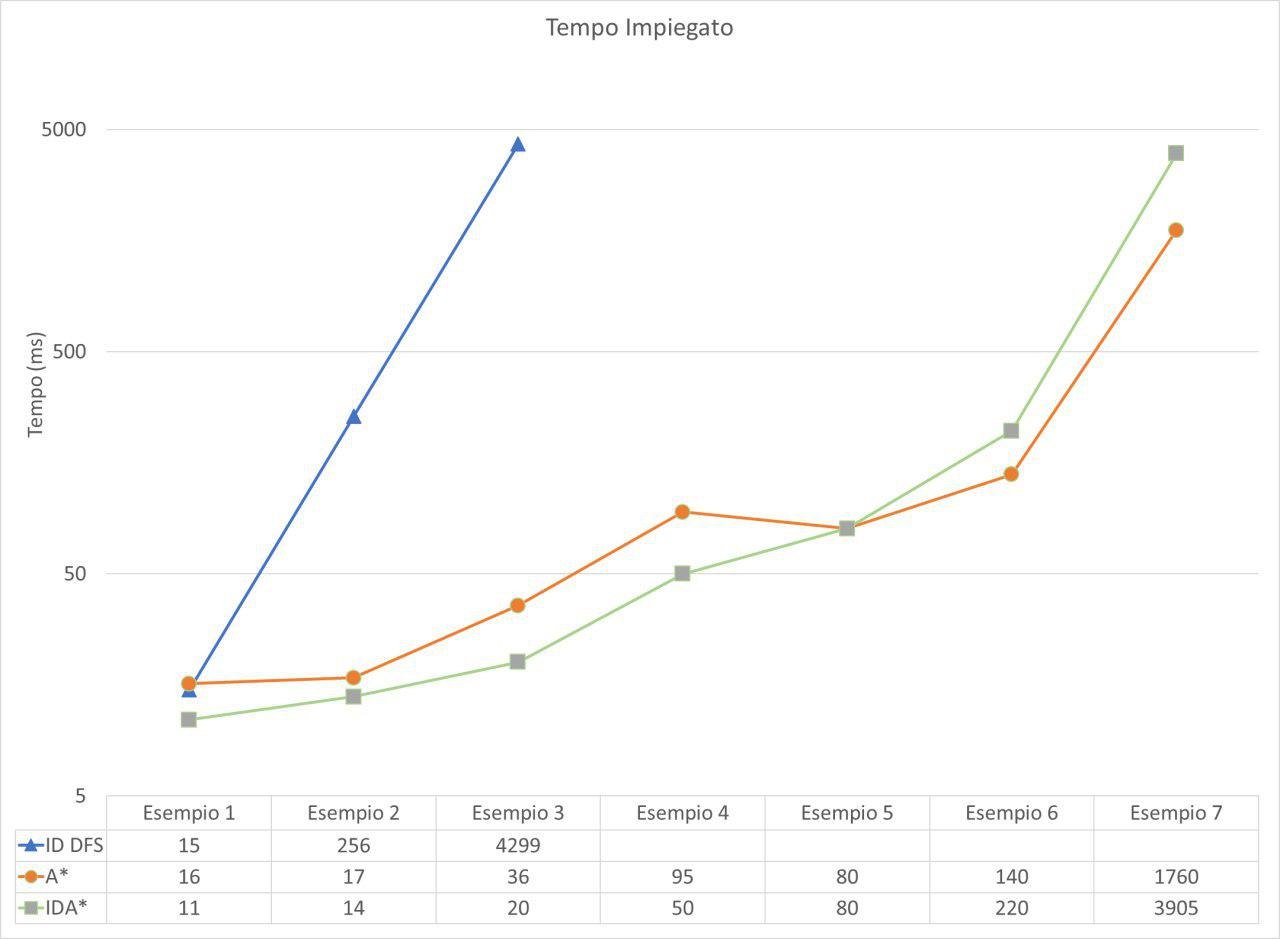
\includegraphics[width=\textwidth]{times}
\vskip 20pt
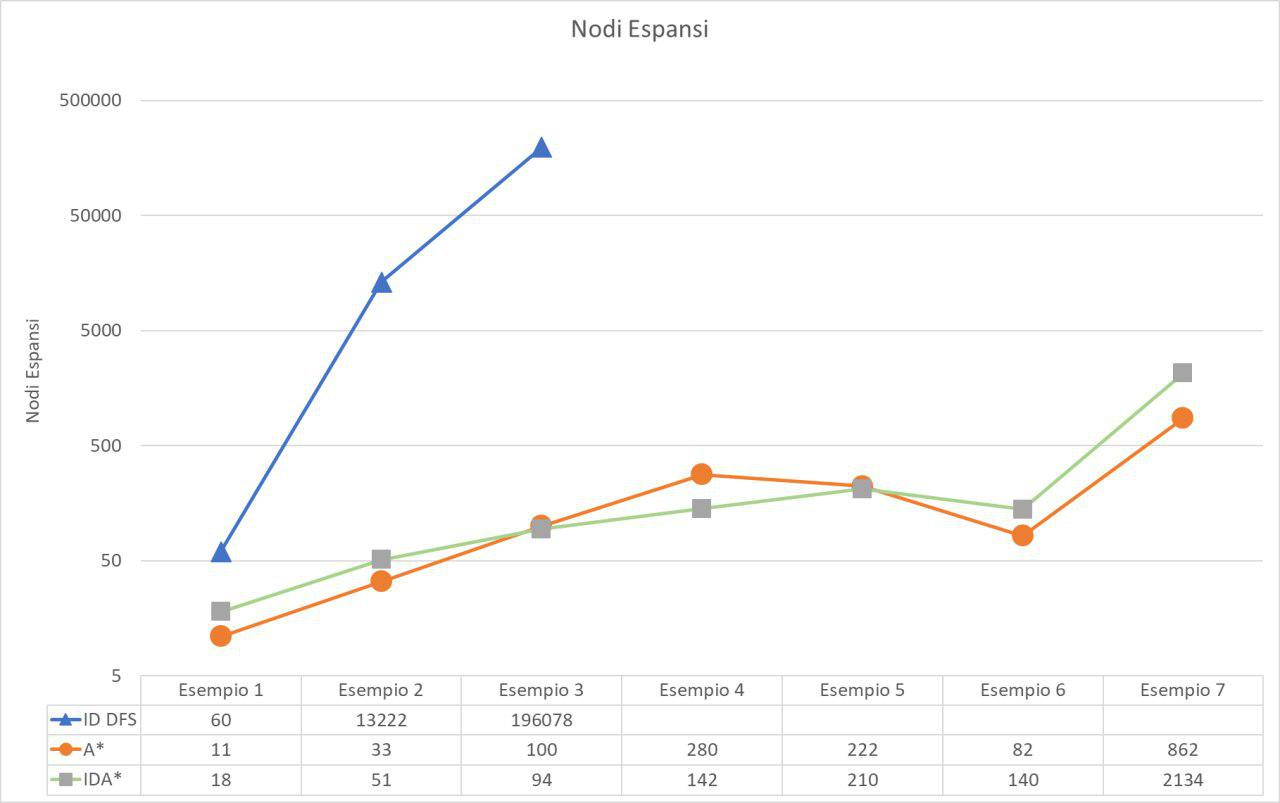
\includegraphics[width=\textwidth]{expanded}
\caption{Confronto fra i diversi algoritmi in termini di tempo impiegato e di nodi espansi. Dati relativi al modello di transizione A e all'euristica B.}
\label{normal_compare}
\end{figure}

\noindent\textbf{Iterative Deepening DFS}\\
L'algoritmo  riesce a risolvere i primi 3 esempi in tempo accettabile. Tuttavia, già dal secondo caso in poi si può notare che il numero di nodi espansi è estremamente maggiore rispetto a quello di A* e IDA*. Il rapido aumento della complessità fa sì che il quarto esempio non possa essere risolto da ID DFS in tempi ragionevoli: l'algoritmo è stato arrestato forzatamente dopo una decina di minuti.\\

\noindent\textbf{\textbf{A\textsuperscript{*}}}\\
Prestazioni migliori si hanno con A*, che risolve efficientemente i primi 6 esempi; l'esempio numero 7 viene risolto dopo pochi secondi di attesa. Non è stato invece possibile risolvere l'esempio 8 in quanto ha portato ad un saturamento totale della RAM disponibile.
Se confrontato con gli altri due algoritmi implementati, il vantaggio principale di A* consiste nel numero di nodi espansi, che in linea di massima risulta inferiore. Questo è in accordo con quanto previsto dalla teoria: A* infatti non soffre di un problema comune a ID DFS e IDA*, ovvero l'espansione ripetuta degli stessi nodi (durante iterazioni successive). Tuttavia, dover mantenere contemporaneamente in memoria tutti i nodi appartenenti alla frontiera (open list) e tutti i nodi già visitati (closed list) rappresenta, all'atto pratico, un limite non trascurabile.\\

\noindent\textbf{\textbf{IDA\textsuperscript{*}}}\\
Se per A* il problema primario è l'eccessiva occupazione della memoria, per IDA* anche il tempo impiegato nella ricerca di una soluzione ottima diventa una criticità rilevante. L'esempio 8 in questo senso risulta emblematico: infatti, in questo specifico caso l'euristica sembra sottostimare notevolmente il costo reale, e ciò costringe l'algoritmo a ritentare molte volte la ricerca a profondità via via maggiori. Così facendo, si spreca un notevole quantitativo di tempo espandendo ripetutamente gli stessi nodi ad ogni nuova iterazione. Tuttavia a differenza di A* (che satura la RAM disponibile piuttosto rapidamente) si è potuto osservare che, prima di fallire a causa della carenza di memoria, IDA* riesce a raggiungere una profondità di 46 (si ricordi che l'euristica B fornisce una stima di soli 34 passi). Il fatto che anche IDA* esaurisca la memoria disponibile è in un certo senso inaspettato: trattandosi di una particolare ricerca in profondità, il numero di nodi che è necessario tenere in memoria è lineare nella profondità della soluzione. Per ciascun livello infatti vengono generati e memorizzati solo i successori del nodo corrente, e la ricerca prosegue in modo ricorsivo dal più promettente di questi. In più, si deve tener conto dei nodi incontrati lungo uno specifico cammino per evitare di considerare nuovamente stati già visitati. Lo spazio occupato quindi non sembra essere eccessivo, almeno a livello teorico. Pertanto, l'ipotesi più accreditata è che l'elevato consumo di memoria sia in parte dovuto all'interprete Prolog, il quale deve presumibilmente memorizzare e gestire strutture dati piuttosto complesse per supportare il suo caratteristico modello di calcolo.

\subsection{Confronto fra modelli di transizione}

Gli esperimenti sono stati quindi ripetuti adottando il modello di transizione B; il numero di pilastri disponibili è stato fissato a 3 in tutti i casi. È facile verificare che un tale numero di pilastri permette di risolvere qualsiasi istanza del problema, anche se le restrizioni rendono molto più difficoltosa la ricerca della soluzione ottimale. In figura \ref{pillar_compare} sono riportati i risultati ottenuti per i primi 4 esempi; i casi più complessi hanno richiesto uno sforzo computazionale eccessivo, soprattutto in termini di memoria occupata, e non è stato possibile risolverli.

\begin{figure}[h]
\centering
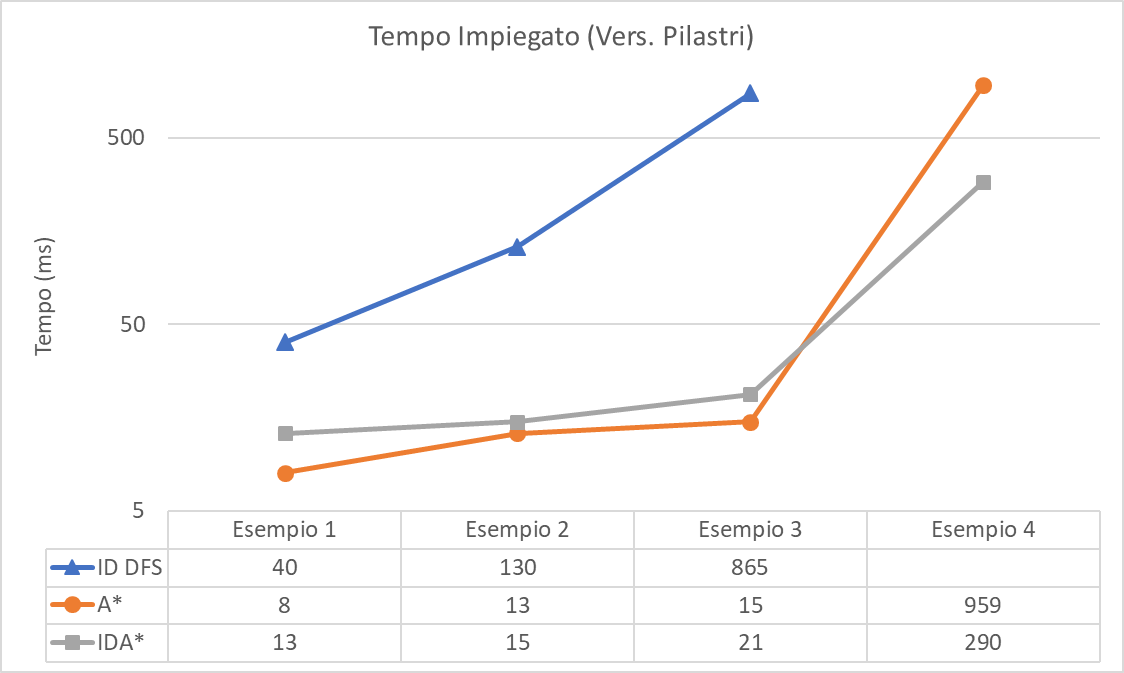
\includegraphics[width=\textwidth]{pillar_times}
\vskip 20pt
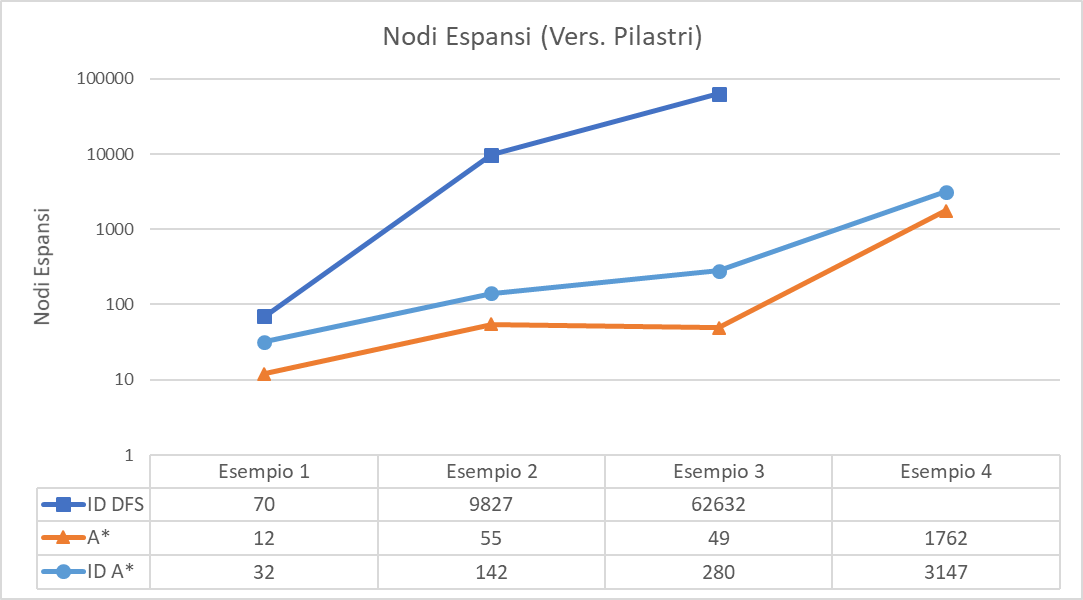
\includegraphics[width=\textwidth]{pillar_expanded}
\caption{Confronto fra i diversi algoritmi in termini di tempo impiegato e di nodi espansi. Dati relativi al modello di transizione B (considerando disponibili 3 pilastri) e all'euristica B. }
\label{pillar_compare}
\end{figure}

\subsection{Confronto fra euristiche}

L'ultimo confronto che riportiamo riguarda le due euristiche implementate. È stato selezionato uno dei due algoritmi più performanti (IDA*) e sono state paragonate le prestazioni nei due casi. L'euristica A, decisamente meno informata, rallenta così tanto la ricerca da rendere impossibile la trattazione di alcuni casi che, ricorrendo all'euristica B, vengono risolti con uno sforzo tutto sommato ridotto. La figura \ref{heuristic_compare} riporta i risultati ottenuti per i primi quattro esempi, gli unici che è stato possibile testare in tempi ragionevoli: una ulteriore conferma di quanto la bontà dell'euristica scelta sia in grado di influenzare significativamente le prestazioni di un algoritmo di ricerca informato. 

\begin{figure}[h]
\centering
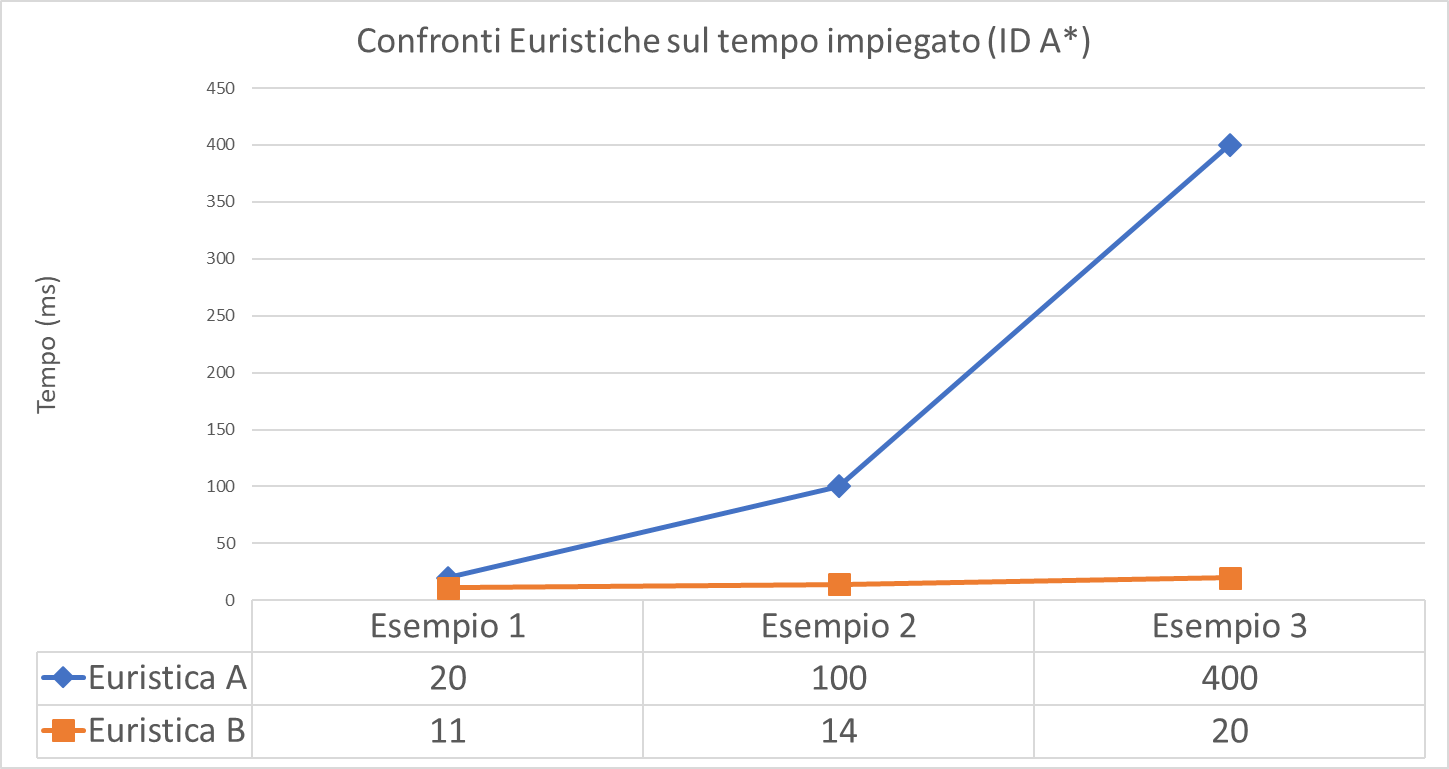
\includegraphics[width=\textwidth]{heuristic_times}
\vskip 20pt
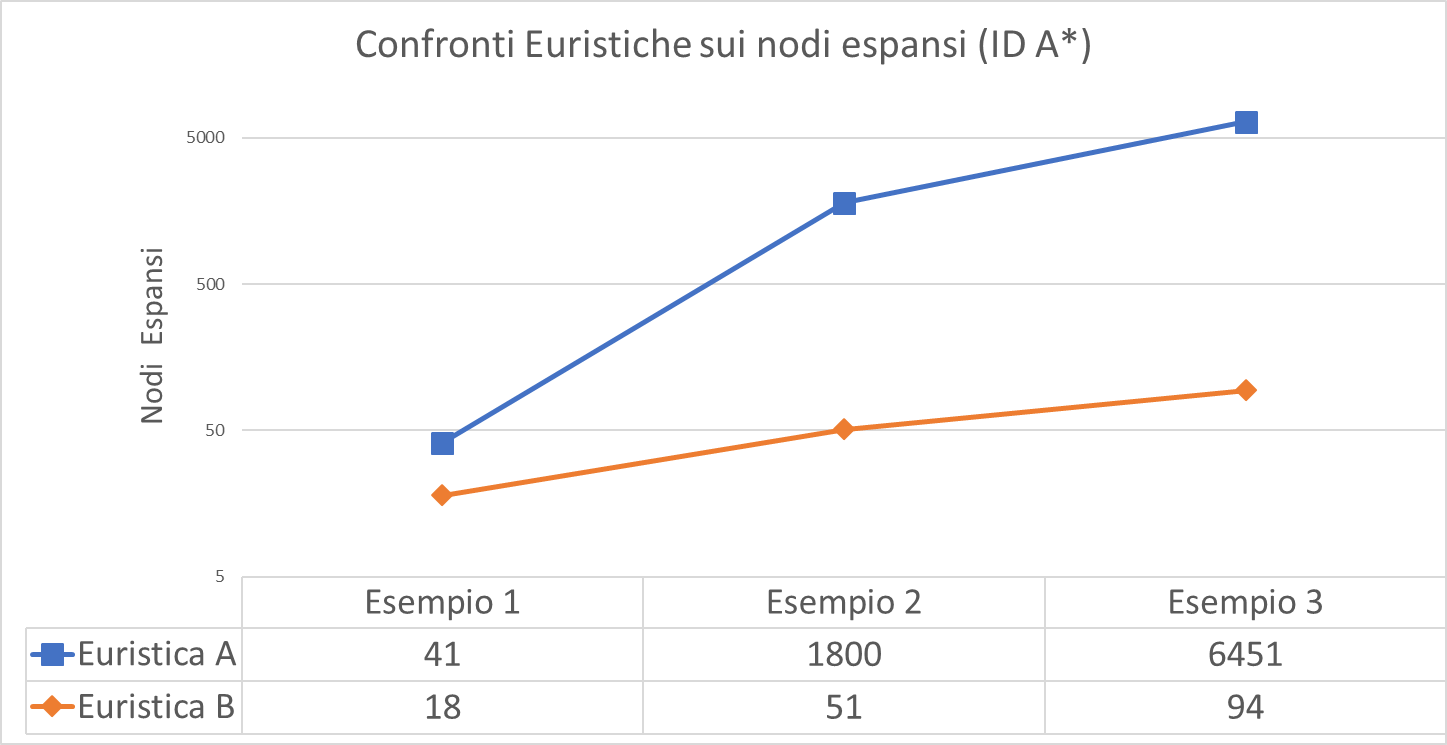
\includegraphics[width=\textwidth]{heuristic_expanded}
\caption{Confronto delle due euristiche realizzate in termini di tempo impiegato e di nodi espansi da uno specifico algoritmo (IDA*)}
\label{heuristic_compare}
\end{figure}
